% Controllable history-taking agent: the LLM handles language; state, policy
% and constraints stay explicit.
% Build: tectonic agent-architecture.tex  ->  agent-architecture.pdf
% The PDF is used by the slides; a PNG export is used by the project page.
\documentclass[tikz,border=6pt]{standalone}
\usepackage[T1]{fontenc}
\usepackage{lmodern}
\usepackage{amsmath,amssymb}
\usetikzlibrary{positioning,arrows.meta}

\definecolor{DEEblue}{RGB}{18,79,135}
\definecolor{boxfill}{RGB}{232,240,248}
\definecolor{alertline}{RGB}{214,120,32}
\definecolor{alertfill}{RGB}{255,242,228}

\begin{document}
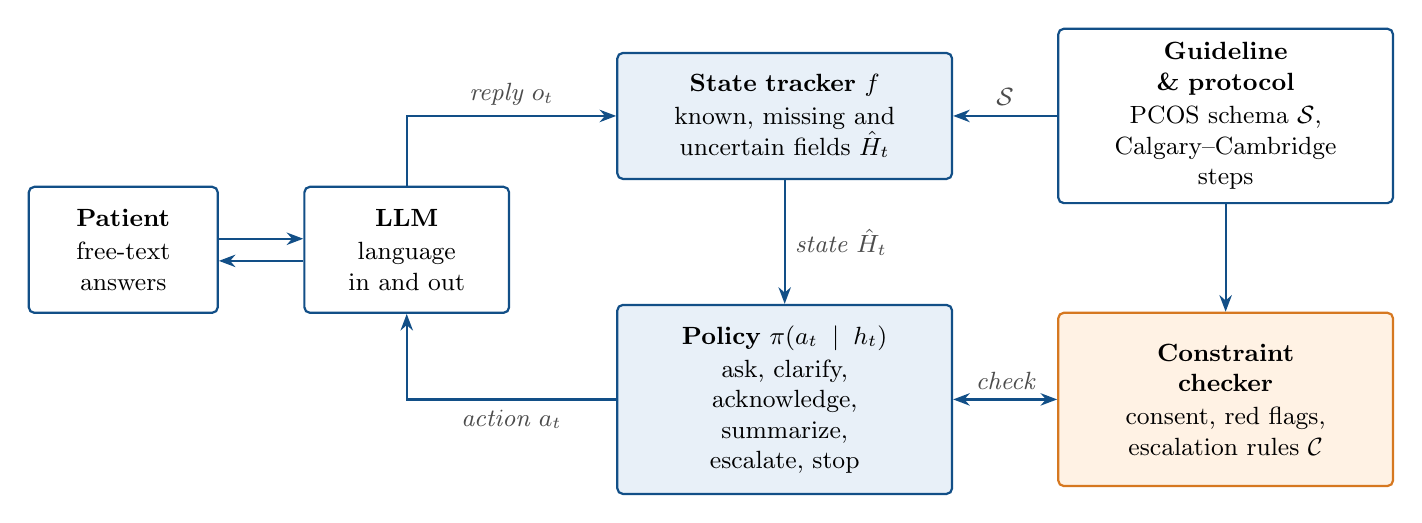
\begin{tikzpicture}[
  font=\small,
  box/.style={draw=DEEblue, thick, rounded corners=2pt, fill=white,
              align=center, inner sep=5pt},
  core/.style={box, fill=boxfill},
  safety/.style={box, draw=alertline, fill=alertfill},
  arr/.style={-{Stealth[length=6pt]}, thick, DEEblue},
  lbl/.style={font=\small\itshape, text=black!70},
]

% Nodes
\node[box, minimum width=2.4cm, minimum height=1.6cm] (patient) at (0,0)
  {\textbf{Patient}\\[1pt]free-text\\answers};
\node[box, minimum width=2.6cm, minimum height=1.6cm] (llm) at (3.6,0)
  {\textbf{LLM}\\[1pt]language\\in and out};
\node[core, text width=3.9cm, minimum height=1.6cm] (state) at (8.4,1.7)
  {\textbf{State tracker $f$}\\[1pt]known, missing and\\uncertain fields $\hat{H}_t$};
\node[core, text width=3.9cm, minimum height=2.4cm] (policy) at (8.4,-1.9)
  {\textbf{Policy $\pi(a_t \mid h_t)$}\\[1pt]ask, clarify,\\acknowledge,\\summarize,\\escalate, stop};
\node[box, text width=3.9cm, minimum height=2.2cm] (guide) at (14.0,1.7)
  {\textbf{Guideline\\\& protocol}\\[1pt]PCOS schema $\mathcal{S}$,\\Calgary--Cambridge\\steps};
\node[safety, text width=3.9cm, minimum height=2.2cm] (check) at (14.0,-1.9)
  {\textbf{Constraint\\checker}\\[1pt]consent, red flags,\\escalation rules $\mathcal{C}$};

% Patient <-> LLM
\draw[arr] ([yshift=4pt]patient.east) -- ([yshift=4pt]llm.west);
\draw[arr] ([yshift=-4pt]llm.west) -- ([yshift=-4pt]patient.east);

% LLM -> state tracker (reply)
\draw[arr] (llm.north) |- node[lbl, above, pos=0.75] {reply $o_t$} (state.west);

% Guideline -> state tracker (schema)
\draw[arr] (guide.west) -- node[lbl, above] {$\mathcal{S}$} (state.east);

% State tracker -> policy
\draw[arr] (state.south) -- node[lbl, right] {state $\hat{H}_t$} (policy.north);

% Policy -> LLM (action)
\draw[arr] (policy.west) -| node[lbl, below, pos=0.25] {action $a_t$} (llm.south);

% Policy <-> constraint checker
\draw[{Stealth[length=6pt]}-{Stealth[length=6pt]}, thick, DEEblue]
  (policy.east) -- node[lbl, above] {check} (check.west);

% Guideline -> constraint checker
\draw[arr] (guide.south) -- (check.north);

\end{tikzpicture}
\end{document}
